\section{Results}
All numbers are means over two seeds (random labeled/unlabeled pools); a third seed was started but not completed, so the standard deviations are over $n{=}2$ and are only a rough indication of variability. Zero-shot results are deterministic given the prompts.

\subsection{Accuracy versus annotation budget}
Table~\ref{tab:main} and Fig.~\ref{fig:curves} give the central result: the best strategy depends on the domain.

\textbf{Construction-PPE (weak zero-shot fit).} The zero-shot teacher reaches only 23.6 mAP$_{50}$ because half of the label space (absence classes such as no\_helmet) is not expressible as a noun phrase. Fine-tuning on just $N{=}10$ labeled images (about 14 minutes of annotation under our default cost model) already exceeds it (27.4), and accuracy rises steadily to 41.1 at $N{=}400$. Teacher--student training \emph{without} gold labels reproduces the teacher (22.3 vs.\ 23.6) and does not exceed zero-shot until the mixed pool contains mostly gold labels ($N{=}200$: 30.9; $N{=}400$ is identical to FT by construction, as the pool has no unlabeled images left). Notably, mixing noisy pseudo-labels with $N$ gold labels is \emph{worse} than discarding them: at $N{=}200$, FT on the 200 gold images alone gets 40.6 against 30.9 for TS with 200 additional pseudo-labeled images, i.e., a 9.7-point loss.

\textbf{HomeObjects-3K (strong zero-shot fit).} The label space is made of common nouns and zero-shot reaches 55.3 mAP$_{50}$. No trained student surpasses it at any budget up to $N{=}400$ (FT 28.4, TS 28.4 at $N{=}400$). FT and TS are indistinguishable from $N{\approx}50$ upward, and both are far below the teacher. Here the right decision is to label nothing and deploy the zero-shot detector, or to spend the budget elsewhere.

\begin{table}[t]
\caption{mAP$_{50}$ ($\pm$std over seeds) / mAP$_{50:95}$ (\%) versus the number of labeled images $N$. ``Ann.\ h'' is annotation time under $t_{img}{=}5$\,s, $t_{box}{=}10$\,s. TS at $N{=}0$ uses no manual labels; FT is undefined there. At $N{=}400$ the pool contains no unlabeled images, so TS$\equiv$FT.}
\label{tab:main}
\centering\scriptsize
\setlength{\tabcolsep}{2.5pt}
\begin{tabular}{rrcccc}
\toprule
$N$ & Ann.\ h & FT & TS & TS-cal & seeds\\
\midrule
\multicolumn{6}{l}{\textit{HomeObjects-3K} (zero-shot: mAP$_{50}$ 55.3, mAP$_{50:95}$ 37.0)} \\
0 & 0.00 & -- & 24.8$\pm$0.0 / 14.7 & -- & 1 \\
10 & 0.24 & 12.5$\pm$0.0 / 6.5 & 23.9$\pm$0.0 / 13.9 & 23.9$\pm$0.0 / 13.9 & 1 \\
25 & 0.61 & 19.5$\pm$0.0 / 10.2 & 24.4$\pm$0.0 / 14.6 & 24.4$\pm$0.0 / 14.6 & 1 \\
50 & 1.21 & 25.8$\pm$0.0 / 14.0 & 25.4$\pm$0.0 / 15.3 & 25.4$\pm$0.0 / 15.3 & 1 \\
100 & 2.43 & 25.7$\pm$0.0 / 14.5 & 24.5$\pm$0.0 / 14.6 & 24.5$\pm$0.0 / 14.6 & 1 \\
200 & 4.85 & 26.9$\pm$0.0 / 15.7 & 27.2$\pm$0.0 / 16.3 & 27.2$\pm$0.0 / 16.3 & 1 \\
400 & 9.71 & 28.6$\pm$0.0 / 17.0 & 28.6$\pm$0.0 / 17.0 & 28.6$\pm$0.0 / 17.0 & 1 \\
\hline
\multicolumn{6}{l}{\textit{Construction-PPE} (zero-shot: mAP$_{50}$ 23.6, mAP$_{50:95}$ 8.4)} \\
0 & 0.00 & -- & 22.3$\pm$0.2 / 7.9 & -- & 2 \\
10 & 0.24 & 27.4$\pm$0.8 / 11.7 & 23.2$\pm$0.0 / 8.3 & 23.2$\pm$0.0 / 8.3 & 2 \\
25 & 0.59 & 32.6$\pm$0.0 / 14.7 & 24.2$\pm$0.0 / 8.6 & 24.2$\pm$0.0 / 8.6 & 1 \\
50 & 1.19 & 38.6$\pm$0.0 / 17.3 & 25.2$\pm$0.0 / 9.5 & 25.2$\pm$0.0 / 9.5 & 1 \\
100 & 2.37 & 39.7$\pm$0.0 / 18.2 & 26.4$\pm$0.0 / 10.2 & 26.4$\pm$0.0 / 10.2 & 1 \\
200 & 4.74 & 40.4$\pm$0.0 / 19.4 & 30.7$\pm$0.0 / 13.0 & 30.7$\pm$0.0 / 13.0 & 1 \\
400 & 9.49 & 41.2$\pm$0.0 / 19.6 & 41.2$\pm$0.0 / 19.6 & 41.2$\pm$0.0 / 19.6 & 1 \\
\hline

\bottomrule
\end{tabular}
\end{table}

\begin{figure}[t]
\centering
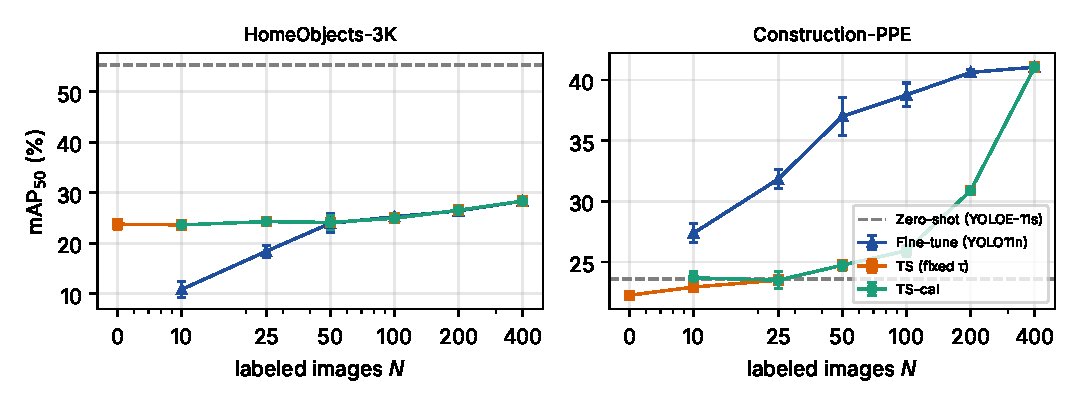
\includegraphics[width=\columnwidth]{figs/learning_curves.pdf}
\caption{mAP$_{50}$ versus labeled images (mean $\pm$ std, 2 seeds). The dashed line is the zero-shot teacher.}
\label{fig:curves}
\end{figure}

\subsection{Is the HomeObjects result a compute artifact?}
Our students are small, trained on CPU at $320$\,px for a fixed budget of 4\,800 image visits, which is likely too little for a strong detector. We therefore re-ran fine-tuning at $N{=}400$ (seed~0 only) with $4\times$ the training visits, and with input size $640$ (Table~\ref{tab:abl}). More compute helps substantially: FT improves from 28.4 to 41.5 (4$\times$ visits) or 40.7 (640\,px) on HomeObjects and from 41.1 to 48.6 on PPE. On HomeObjects the zero-shot detector (55.3) still wins at $N{=}400$, but the gap shrinks from 27 to about 14 points, so we \emph{cannot} claim that zero-shot beats fine-tuning there at convergence, only within our compute budget. We did not run the corresponding ablation for TS or for larger $N$, nor train to convergence, so the crossover for HomeObjects may lie above $N{=}400$ and the absolute numbers of all trained students are lower bounds.

\begin{table}[t]
\caption{Compute sensitivity of FT at $N{=}400$ (mAP$_{50}$ \%; ablations: seed 0 only, run alone on 4 CPU threads; main column: mean of 2 seeds; ``--'': not run).}
\label{tab:abl}
\centering\footnotesize
\begin{tabular}{lcccc}
\toprule
& Main (320\,px, $1\times$) & $4\times$ visits & 640\,px & Zero-shot\\
\midrule
HomeObjects-3K & 28.4 & 41.5 & 40.7 & 55.3 \\
Construction-PPE & 41.1 & 48.6 & -- & 23.6 \\

\bottomrule
\end{tabular}
\end{table}

\subsection{Annotation cost}
Fig.~\ref{fig:cost} plots accuracy against annotation time. On PPE, reaching 75\% of the best FT accuracy observed in our grid (30.8 mAP$_{50}$) takes $N{=}25$ labeled images for FT, about 0.6\,h at $t_{box}{=}10$\,s (0.3\,h at 5\,s, 2.0\,h at 35\,s), whereas TS reaches that level only at $N{=}200$ (4.7\,h). Zero-shot never reaches it. The ranking of strategies does not depend on $t_{box}$, because the cost model is linear in $N$ for all learned strategies; it only rescales the horizontal axis.

\begin{figure}[t]
\centering
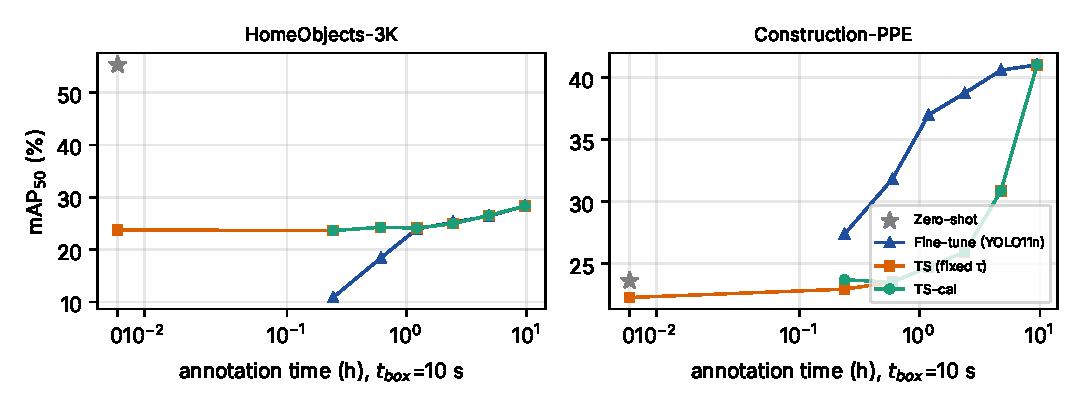
\includegraphics[width=\columnwidth]{figs/cost_accuracy.pdf}
\caption{Accuracy versus annotation time ($t_{box}{=}10$\,s). Zero-shot costs no annotation.}
\label{fig:cost}
\end{figure}

\subsection{Gold-calibrated pseudo-label threshold}
TS-cal selected the default $\tau_0{=}0.25$ in 23 of 24 (dataset, seed, $N$) cases, so for those it is identical to TS by construction. In the single case where it chose a different threshold ($\tau{=}0.10$, PPE, $N{=}10$, seed~1) mAP$_{50}$ rose by 1.5 points, which is within the seed-to-seed variation we observe. Our grid $\{0.1,0.25,0.4\}$ and the F$_1$ criterion thus provide \emph{no measurable benefit} here; the claimed contribution is a mechanism, not an effect we have demonstrated.

\subsection{Strategy selector}\label{sec:selector}
We fit each learned strategy's curve on the pilot budgets $N\in\{10,25,50\}$ of one seed and let the selector choose a strategy for $N\in\{100,200,400\}$, comparing with the strategy that was best in hindsight on the same seed (Table~\ref{tab:sel}; 12 cases: 2 datasets $\times$ 2 seeds $\times$ 3 budgets). Both curve families chose the best strategy in all 12 cases (regret 0), versus a mean regret of 8.3 mAP$_{50}$ points for always using zero-shot, 14.3 for always fine-tuning (and for the rule ``fine-tune once $N\ge100$''), and 18.1 for always using TS. We stress that this evidence is weak: the winner is the same at every budget within each dataset (zero-shot on HomeObjects, FT on PPE) and the cases are strongly correlated, so a perfect score tests extrapolation in a regime where no crossover occurs within $[100,400]$. The selector has not been tested where curves actually cross inside the extrapolation range.

\begin{table}[t]
\caption{Selector evaluated by extrapolating from $N\le50$ to $N\in\{100,200,400\}$. Hit: chosen strategy within 0.5 point of best (\%); regret in mAP$_{50}$ points (mean over 12 cases) for the selector and for fixed policies.}
\label{tab:sel}
\centering\scriptsize
\setlength{\tabcolsep}{2.5pt}
\begin{tabular}{llrrrrrrr}
\toprule
curve & strategies & cases & hit & selector & ZS & TS & FT & FT$_{N\ge100}$\\
\midrule
loglin & ZS/TS/FT & 12 & 100 & 0.00 & 8.26 & 18.11 & 14.33 & 14.33 \\
power & ZS/TS/FT & 12 & 100 & 0.00 & 8.26 & 18.11 & 14.33 & 14.33 \\

\bottomrule
\end{tabular}
\end{table}

\subsection{How many labeled images are needed to measure zero-shot accuracy?}
A budget-aware decision requires an estimate of the zero-shot detector's accuracy, which needs labeled data. Table~\ref{tab:pilot} reports the error of mAP$_{50}$ estimated on a random subset of $n$ labeled images relative to the full evaluation set (200 random subsets). The estimate is noisy and biased upward for small $n$ (subsets contain fewer classes, and rare hard classes are missing): with $n{=}10$ the mean absolute error is 7--9 points; $n{=}50$ brings it to 2.5--3.4; and $n{=}100$ to 1.4--2.6. For ordering zero-shot against FT at $N{=}100$ the pilot ordering agreed with the full-set ordering in $\ge$99.5\% of subsets for every $n$, but the gaps there (about 15 points on PPE and 30 on HomeObjects) are large relative to this error; for closer pairs a larger pilot set would be needed.

\begin{table}[t]
\caption{Error of zero-shot mAP$_{50}$ measured on $n$ labeled pilot images: mean absolute error / mean bias (points).}
\label{tab:pilot}
\centering\footnotesize
\begin{tabular}{lcccc}
\toprule
 & $n{=}10$ & 25 & 50 & 100\\
\midrule
HomeObjects-3K & 6.9 / +4.1 & 4.9 / +2.3 & 3.4 / +1.0 & 2.6 / +0.9 \\
Construction-PPE & 9.3 / +8.4 & 5.0 / +3.7 & 2.5 / +1.5 & 1.4 / +0.6 \\

\bottomrule
\end{tabular}
\end{table}

\subsection{Inference cost}
Table~\ref{tab:speed} shows the deployment benefit of distillation: the YOLO11n student is 3.9--4.6$\times$ faster than the YOLOE-11s teacher on CPU at its trained resolution (and about 2.3--2.6$\times$ at 640\,px), but on HomeObjects this speed costs roughly 27--31 mAP$_{50}$ points in our budget-limited setting.

\begin{table}[t]
\caption{Median CPU latency per image (ms, batch 1, 4 threads).}
\label{tab:speed}
\centering\footnotesize
\begin{tabular}{lcccc}
\toprule
 & Teacher 640 & Student 640 & Student 320 & Speed-up\\
\midrule
HomeObjects-3K & 183 & 79 & 47 & 3.9$\times$ \\
Construction-PPE & 197 & 75 & 43 & 4.6$\times$ \\

\bottomrule
\end{tabular}
\end{table}

\section{Discussion}
\textbf{Practical guidance.} Three observations hold in both datasets and are likely to transfer. First, the label set matters more than the budget: when class names are natural-language nouns that the teacher recognizes, zero-shot is a strong baseline that small labeled sets do not beat; when classes encode domain semantics (here, absence of equipment), a few tens of labels beat zero-shot. Second, a few labeled images are valuable twice: they supervise FT, and they let one \emph{measure} the zero-shot detector (error 2.5--3.4 points at 50 images) before committing to any larger annotation spend. Third, pseudo-labels are not free supervision: they matched the teacher at best, and mixing them with scarce gold labels hurt. A practitioner who has even 25--50 gold images in a domain where the teacher is weak should fine-tune on them rather than pool them with noisy pseudo-labels.

\textbf{Relation to prior work.} Our observation that a teacher-trained student can match its teacher on PPE agrees with reports that auto-labeling can replace manual labels~\cite{son2024teacherstudent,abid2025waste}, but our HomeObjects result (student far below the teacher at small compute) and the harm from mixing at PPE $N{=}200$ show that this depends on teacher quality and training budget, in line with the large zero-shot failures documented on Roboflow100-VL~\cite{robicheaux2025rf100vl}.

\section{Limitations}
This is a small-scale study and its conclusions should be read accordingly. (i)~Two datasets and one teacher--student pair (YOLOE-11s $\rightarrow$ YOLO11n); we did not evaluate Grounding~DINO, OWLv2, YOLO-World, or retail data (RPC), which motivated the project but was not accessible. (ii)~All trained students are compute-limited (CPU, 320\,px, 4\,800 image visits); the ablation shows this changes absolute numbers by 8--13 points and may move crossover points, so the HomeObjects ``zero-shot wins'' result is specific to this budget. (iii)~Two seeds only, with $n{=}2$ standard deviations; a third seed was started and discarded unfinished. (iv)~The unlabeled pool has 400 images, so TS and FT coincide at $N{=}400$, and TS is not tested with a large pool, where pseudo-labels may help more. (v)~The annotation-time model ($t_{img}$, $t_{box}$) is assumed, not measured. (vi)~TS-cal showed no measurable effect and the selector evaluation contains no budget range with an actual crossover. (vii)~Prompts were fixed a priori and never tuned; prompt engineering could change the zero-shot baseline, especially for PPE.

\section{Conclusion}
We compared zero-shot detection, pseudo-label distillation, and fine-tuning as a function of the number of labeled images on two domains. The best strategy depended on the domain rather than on the budget alone: zero-shot won on a common-noun label space up to 400 labeled images in our (compute-limited) setting, while on a domain-specific label space as few as 10 labeled images made fine-tuning better than zero-shot, and pseudo-labels from the weak teacher were never better than gold labels. A small labeled pilot set can reliably rank strategies when their gaps exceed a few points, and learning-curve extrapolation chose the right strategy in all of our (low-difficulty) test cases. Larger-scale validation with stronger teachers, converged students, retail data, and settings with genuine crossovers is needed before the selector can be recommended in practice.

\section*{Reproducibility}
Code, per-image evaluation statistics, and all raw results are in the accompanying repository (\texttt{scripts/run\_experiments.py}, \texttt{scripts/analyze.py}).

\bibliographystyle{IEEEtran}
\bibliography{refs}
\end{document}
